\documentclass[11pt,titlepage]{article}
\usepackage{fullpage}
\usepackage{amsmath}
\usepackage{amssymb}
\usepackage{tikz}
\usetikzlibrary{shapes,arrows,positioning,calc}
\usepackage{float}
\restylefloat{table}
\usepackage{array}
\tikzset{
	block/.style = {draw, fill=white, rectangle, minimum height=3em, minimum width=3em},
	sum/.style = {draw, fill=white, circle, node distance=1cm},
	input/.style = {draw=none},
	output/.style = {draw=none},
	coord/.style = {coordinate}
}

\author{Rane Brown \\ Kate Schneider}
\title{ECEN 4638: Lab X}
\date{\today}

\begin{document}
\maketitle

\section*{Purpose}
	Lab X is designed to review the basics of feedback control. This will be accomplished through a series of procedures that analyze a cruise control system. The end goal of this project is to gain enough knowledge and background information to create a feasible control solution for use with the torsion disk system.

\section*{Background}
	Feedback is important in nature and technology. Without feedback life as we know it would not exist and the technological marvels that exits today would not be possible. There are numerous example of existing feedback systems but a few of the most important are listed below.

	\subsection*{E1}
		\begin{enumerate}
			\item Airplane: The autopilot can be set to maintain a level orientation at a given altitude. Disturbances in the air may cause the wings to dip and this movement is read by a gyroscope. The information from the gyroscope is read by the control system and adjustments are made to the ailerons to bring the plane back to a level orientation.
			\item Thermostat: The user can select a desired temperature and the thermostat will compare this value to the measured temperature. If hot air from outside the house raises the temperature above the set value the ac will be activated. 
			\item Climate change: Greenhouse gases increase the Earth's temperature and this rise in temperature increases water vapor in the air. The increase in water vapor further increases the Earth's temperature. In addition, there is ice albedo feedback where the reduction of ice due to melting reduces the amount of reflected radiation and therefore the surface temperature rises which leads to further ice melting.
			\item Metabolism: The metabolism of an animal is adjusted depending on food intake. As the food intake decreases the metabolism slows and vice versa.
		\end{enumerate}

\section*{Procedure}
	A simple example of a feedback system that has wide spread real world application is cruise control. The most common example of this appears in vehicles. The driver can set the desired speed and the feedback system will maintain that speed in the presence of disturbances such as wind and hills. \\

	\begin{figure}[!htb]
	\centering
	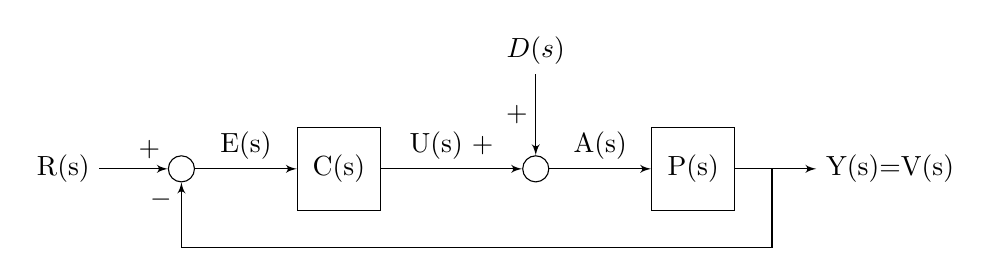
\begin{tikzpicture}[auto, node distance=2cm,>=latex']
		\node [input, name=rinput] (rinput) {R(s)};
		\node [sum, right of=rinput, node distance=1.5cm] (sum1) {};
		\node [coord, below of=sum1, node distance=1cm] (fdbk1) {};
		\node [block, right of=sum1] (controller) {C(s)};
		\node [sum, right of=controller, node distance=2.5cm] (sum2) {};
		\node [block, right of=sum2, node distance=2cm] (plant) {P(s)};
		\node [coord, right of=plant, node distance=1cm] (fdbk2) {};
		\node [coord, below of=fdbk2, node distance=1cm] (fdbk3) {};
		\node [input, above of=sum2, node distance=1.5cm] (disturbance) {$D(s)$};
		\node [output, right of=plant, node distance=2.5cm] (output) {Y(s)=V(s)};
		\draw [->] (rinput) -- node[xshift=.2cm]{$+$} (sum1);
		\draw [->] (disturbance) -- node[xshift=-.5cm]{$+$} (sum2);
		\draw [->] (sum1) --node {E(s)} (controller);
		\draw [->] (controller) -- node{U(s) $+$} (sum2);
		\draw [->] (sum2) -- node{A(s)} (plant);
		\draw [->] (plant) -- node {}(output);
		\draw [-] (fdbk2) -- (fdbk3);
		\draw [-] (fdbk3) -- (fdbk1);
		\draw [->] (fdbk1) -- node[yshift=.2cm]{$-$} (sum1);
	    \end{tikzpicture}
	\caption{Cruise Control Feedback System} \label{fig:block}
	\end{figure}

	\noindent As seen in Figure \ref{fig:block} there are two inputs signal to the cruise control feedback system: the reference $R(s)$ and the disturbance $D(s)$. There is one output signal $Y(s)$ for this system but there are many other points of interest as labeled in Figure \ref{fig:block}. With these signals many useful transfer functions can be derived that will help in the selection of an appropriate controller $C(s)$. The selection for $C(s)$ is dependent on many factors including desired rise time, settle time, overshoot, and steady state error. \\

	\begin{table}[!htb]
		\centering
		\begin{tabular}{|m{5cm}|m{9cm}|} 
		\hline
		Signal or Transfer Function & Description \\ 
		\hline
		$Y(s)=V(s)$ & vehicle velocity \\
		\hline
		$R(s)$ & reference velocity \\
		\hline
		$E(s)=R(s)-Y(s)$ & velocity error \\
		\hline
		$U(s)$ & controller output \\
		\hline
		$A(s)$ & vehicle acceleration \\
		\hline
		$D(s)$ & disturbance acceleration \\
		\hline 
		$P(s)=\frac{k}{s+b}$ & plant \textbf{transfer function} \\
		\hline 
		$C(s)$ & controller \textbf{transfer function} \\
		\hline 
		$H_{yr}(s)=\frac{Y(s)}{R(s)}$ & closed loop \textbf{transfer function} from $R(s)$ to $Y(s)$ \\
		\hline 
		$H_{yd}(s)=\frac{Y(s)}{D(s)}$ & closed loop \textbf{transfer function} from $D(s)$ to $Y(s)$ \\
		\hline 
		$H_{ur}(s)=\frac{U(s)}{R(s)}$ & closed loop \textbf{transfer function} from $R(s)$ to $U(s)$ \\
		\hline
		$H_{ud}(s)=\frac{U(s)}{R(s)}$ & closed-loop \textbf{transfer function} from $D(s)$ to $U(s)$ \\
		\hline
		\end{tabular}
		\caption{Signals and Transfer Functions} \label{table:SaTF}
		\end{table}

		\noindent Table \ref{table:SaTF} provides definitions for the signals and transfer functions that will be used for the remainder of Lab X. Common notation will be to exclude the $(s)$ when writing equations i.e. $R(s)$ will be represented as $R$.

	\subsection*{E2}
		The first transfer of function of interest is from the input $R$ to the output $Y$. This transfer function can be found by setting the disturbance $D$ to zero and chasing the signals from figure \ref{fig:block}. The reason it is possible to set $D=0$ and find an individual piece of the overall transfer function is due to the principle of superposition.
		\begin{equation}
			H_{yr}=\frac{Y}{R}=\frac{C*P}{1+C*P}
		\end{equation}
		\begin{equation} \label{eq:Hyr}
			\mbox{ Substituting in for P yields: } H_{yr}=\frac{C*k}{(s+b)+C*k}
		\end{equation} 
	
	\subsection*{E3}
		A second transfer function of interest is from the disturbance $D$ to the output $Y$. Once again, the principle of superposition can be utilized to find the desired transfer function $H_{yd}$ by setting $R=0$. In this case, it can be seen that ``$b\geq 0$ indicates dissipation (friction, wind, etc...) and $k\geq 0$ indicates that a positive command should result in an increase in velocity''
		\begin{equation}
			H_{yd}=\frac{Y}{D}=\frac{P}{1+C*P}
		\end{equation}
		\begin{equation} \label{eq:Hyd}
			\mbox{ Substituting in for P yields: } H_{yd}=\frac{k}{(s+b)+C*k}
		\end{equation}

	\subsection*{E4}
		The purpose of a feedback control system is to design the controller $C$ in such a manner that the output behaves as desired. A controller that commands an acceleration proportional to the velocity error is proportional feedback. $$u(t)=k_p(r(t)-y(t))$$ This is an example of a negative feedback system. For sections E4-E8 a proportional controller will be used: $$C_p=k_p$$ Substituting this proportional controller into equations \ref{eq:Hyr} and \ref{eq:Hyd} gives the following transfer functions.
		\begin{equation} \label{eq:propHyr}
			 H_{yr}=\frac{k_p*k}{(s+b)+k_p*k}
		\end{equation}
		\begin{equation} \label{eq:propHyd}
			H_{yd}=\frac{k}{(s+b)+k_p*k}
		\end{equation}
		Examination of these two transfer functions shows that there are no zeros in either case. The poles of the two transfer functions are identical at $s=-b-k_p*k$. In order for the system to be BIBO stable there can be no right-half-plane poles or zeros. For this to be true $$k_p>\frac{-s-b}{k}$$

	\subsection*{E5}
			

	\subsection*{E6}

	\subsection*{E7}

	\subsection*{E8}

	\subsection*{E9}

	\subsection*{E10}

	\subsection*{E11}

	\subsection*{E12}

	\subsection*{E13}

	\subsection*{E14}

	\subsection*{E15}

	\subsection*{E16}

	\subsection*{E17}

\end{document}